\setcounter{footnote}{0}
\setcounter{section}{0}
\setcounter{ExNo}{0}
\begin{center}
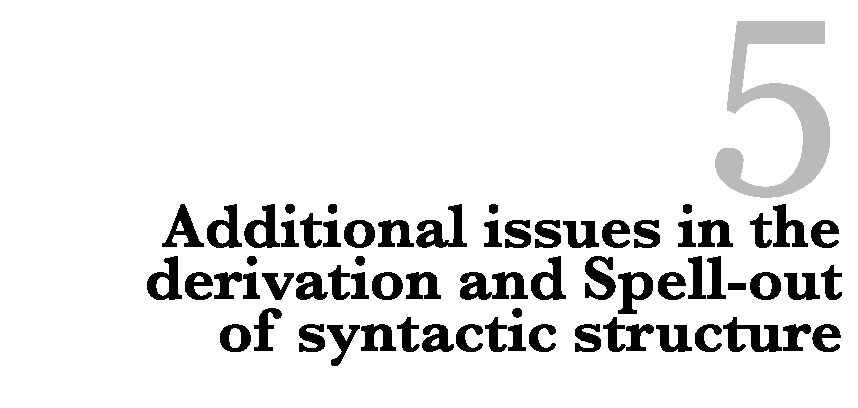
\includegraphics{chapter5.eps}
\end{center}
\section*{}
\addcontentsline{toc}{section}{\Large{Chapter 5: Additional issues in the derivation and Spell-out of syntactic structure}}
\section{Introduction}
In this final chapter, we will look at a few issues that have been left unresolved in the previous analyses of downward movement. The goal of the following sections is to simply explore these issues and propose avenues of research that may lead us to eventually find solutions to the questions that arise. In Section 2, we revisit the Spell-out status of phrasal specifiers of phase projections, and I suggest that it is possible to devise of a model of cyclic Spell-out in which the phase head, its complement, and its specifier all undergo Spell-out on the same cycle. In Section 3, I note an apparent problem of the triggering model of Spell-out for covert phrasal movement. In particular, covert movement to Spec{\it v}P after merger of T appears to violate the constraint that all mergers target the root constituent (i.e.\ some version of the Extension Condition). I will suggest that a dual workspace model of syntactic derivation---as in \citeauthor{nunes2001} (\citeyear{nunes2001}, \citeyear{nunes2004})---provides a possible solution to this problem, with the added implication that Lowering is a sideward movement between derivational phase workspaces. Section 4 provides a brief, overall conclusion to the thesis and suggests some additional areas for future research.

\section{Ternary Spell-out Hypothesis}\label{tern_spellout_sec}
In the previous chapters I proposed the {\it Phase Head Impenetrability Condition} (PHIC), which requires that the head of a phase be included in the Spell-out domain of that phase, contra other models of Spell-out in which only the phrasal complement of the phase head undergoes Spell-out (e.g.\ \citenop{chomsky2001}, \citenop{nissenbaum2000}). However, I argued that this spelled-out head is still accessible due to an edge condition on phases; namely, higher narrow syntactic elements may target the least embedded (i.e.\ ``topmost'') feature(s) of a spelled-out phase {\it n} any time before Spell-out of phase {\it n+1}. Thus, the least embedded feature(s) of a phase head---in other words, the feature(s) of the phase head itself---can be targeted for narrow syntactic movements.\footnote{Note that I allow for a situation in which multiple features may qualify as the ``least embedded'' features, as long as these are all contained in the phase head itself and not embedded in sub-constituents of that head.}

This raises the question as to whether the same scenario holds for the topmost {\it phrasal} constituent within a phase, i.e.\ the specifier of the phase head. Until now I have remained agnostic as to whether the specifier of a phase is included in the Spell-out domain of that phase. Assuming that the implications of the PHIC with respect to the Spell-out status of phase heads hold, we are left with two options regarding the Spell-out of specifiers: 1) a partial model of Spell-out in which just the phase head and its complement are included in the Spell-out domain, leaving the specifier of the phase intact, or 2) a full model of Spell-out in which the phase head, its complement, and its specifier are all included in the Spell-out domain of the phase.


In choosing between these two models of Spell-out, we should first note that the question of the status of specifiers under Spell-out of a phase becomes somewhat trivial in light of \posscitet{uriagereka1999} multiple Spell-out model. Consider the following data, which illustrate that extraction from a specifier is impossible (i.e.\ \posscitet{huang1982} {\it Condition on Extraction Domain} (CED) effects):

\singlespacing
\begin{quote}
\ex.
\a. Who$_{i}$ did you see [a critic of {\it t}$_{i}$]?
\b. *Who$_{i}$ did [a critic of {\it t}$_{i}$] see you?

\end{quote}
\onehalfspacing
\citet{uriagereka1999} argues that such effects are accounted for if specifiers constitute their own Spell-out domains; i.e., in later terms, all specifiers are phases. In terms of the above example, the subject DP [{\it a critic of who}] is derived and spelled out before it merges to the Spec{\it v}P position, as follows (structures simplified; see the following section for a workspaces model of derivation that allows for such a scenario):

\singlespacing
\begin{quote}
\ex.
\a. Derivation of subject DP:\\\\
\begin{tabular}[t]{lcc}
Narrow syntax & Spell-out & PF\\
 & & \\
\Tree [.DP D\\a [.NP N\\critic [.PP P\\of \qroof{who}.DP ].PP ].NP ] & $\rightarrow$ & [a $^{\wedge}$ critic $^{\wedge}$ of $^{\wedge}$ who]\\
 & & \\
\end{tabular}
\b. Derivation of core {\it v}P:\\\\
\Tree
[.{\it v}P \mbox{[\raisebox{-2pt}{\sc{dp}} \textbf{\textit{a critic of who}}]} [.{\it v}P [.{\it v} {\it v} V$_{i}$\\see ].{\it v} [.VP {\it t}$_{i}$ \qroof{you}.DP ].VP ].{\it v}P ]

\end{quote}
\onehalfspacing
When the subject merges in \Last[b], it is an already spelled-out---and thus impenetrable---domain. Clearly, since subjects may undergo subsequent narrow syntactic movement from Spec{\it v}P to SpecTP, the topmost (i.e.\ least embedded) feature of the phrase in Spec{\it v}P must be visible to higher syntactic constituents. However, the features embedded within these subject phrases are inaccessible. As Uriagereka points out, this not only accounts for the observed CED effects of subjects, but also allows for a simpler analysis of linearization at PF. In particular, the entire subject is analyzed as a single constituent for the purposes of linearization, and therefore it is not necessary to account for the linearization of sub-constituents within the subject with respect to the rest of the structure (e.g.\ {\it who} itself does not need to be linearized with respect to elements in {\it v}P, as would be necessary under an approach to linearization like that in \citenop{kayne1994}).

If Uriagereka is correct that specifiers undergo Spell-out even before they are merged within a phase, then the issue of whether a specifier is sent (again) to PF on the Spell-out cycle of the phase reduces to the following question: is the (atomic) phrase in specifier position linearized with respect to the remainder of the phase on that phase's Spell-out cycle, and, if so, how might higher elements target that specifier for extraction (as a single unit)? I have already argued that the phase head may be targeted as a unit for extraction from the phase after Spell-out, and I now propose that it is possible that the specifier is subject to similar conditions on extraction from the phase. To this end, I suggest the following model of Spell-out (Jon Nissenbaum, p.c.):

\singlespacing
\begin{quote}
\ex. {\it Ternary Spell-out Hypothesis}\\
When a phase is triggered for Spell-out, the phase head, its specifier, and its complement are included in the Spell-out domain. After Spell-out of the phase, only the least embedded phrasal feature(s) (i.e.\ the topmost feature(s) of the phase's specifier) and head feature(s) (i.e.\ the feature(s) of the phase head) are accessible to higher elements.

\end{quote}
\onehalfspacing
As noted in the above definition, a ternary model of Spell-out requires that the least embedded features of both the phase head and the specifier be visible to higher elements; that is, if the specifier is included in the Spell-out domain of a phase, it is necessary that its least embedded feature still be accessible to higher narrow syntactic elements after this Spell-out operation {\it and} that the least embedded feature of the phase head also be accessible to higher elements. In this way, we simply need to modify our edge condition such that both the topmost phrase and head of a phase constitute the edge.\footnote{I will assume that in the case of multiple specifiers, all specifiers are treated equally in terms of their inclusion in the Spell-out domain and their potential for extraction from the phase.} This scenario would allow for extraction of the phase head in the absence of extraction of the specifier, as some have argued is the case in Irish; i.e., the verb undergoes overt head movement to INFL but the subject remains {\it in situ} in Spec{\it v}P \citep{mccloskey1991}. Given the vastly different characteristics of head and phrasal movement, such a dual edge condition is not outside the realm of possibility. On this view, a spelled-out phase consists of three individual, atomized constituents [YP [X WP]]; the highest phrase, the specifier YP, may be targeted for subsequent phrasal movements and the highest head, X, for head movements, in keeping with the stated conditions on feature impenetrability.\footnote{I will assume that extraction of the complement WP is only possible if it moves to the specifier of the phase before Spell-out----i.e., before PF Spell-out in the case of overt movement and before LF Spell-out in cases of covert movement; see \S\ref{covert_mov}.} This model of Spell-out essentially only modifies the view of the specifier position of a phase as an ``escape hatch'' for movement. In particular, the specifier of a phase constituent is an escape hatch for movement not because it lies outside the Spell-out domain of the phase, but rather because it is contained in the portion of the Spell-out domain that is still accessible to higher elements due to an edge condition on phases.

Such a model of Spell-out has some important consequences for certain syntactic phenomena. For example, this model supports an adjunct analysis of floating quantifiers, rather than a constituent analysis. Consider the following basic example of Q-float under a constituent analysis (e.g.\ \citenop{sportiche1988}):

\singlespacing
\begin{quote}
\ex.
\a. [\raisebox{-3pt}{\sc{qp}} All [\raisebox{-3pt}{\sc{dp}} the students]]$_{i}$ have {\it t}$_{i}$ left.
\b. [\raisebox{-3pt}{\sc{dp}} The students]$_{i}$ have [\raisebox{-3pt}{\sc{qp}} all {\it t}$_{i}$ ] left.

\end{quote}
\onehalfspacing
According to \citeauthor{sportiche1988}, the semantic equivalence of the above examples implies that they are derived from the same underlying structure, namely that the QP [{\it all~the~students}] forms an underlying constituent in both. Under such a constituent analysis, the subject QP is first merged in Spec{\it v}P and then, in the Q-float example \Last[b], the embedded DP [{\it the students}] is extracted to SpecTP. Thus, it is argued that floated quantifiers arise when a movement operation has optionally targeted the complement of the quantifier, rather than the entire QP itself. Under Uriagereka's multiple Spell-out analysis of CED effects, such a derivation is impossible; that is, [{\it all the students}] constitutes an impenetrable domain when it is merged in Spec{\it v}P. However, we might conjecture, as argued by Sportiche, that the embedded DP undergoes movement to SpecQP before extraction to SpecTP in a Q-float construction. Under Uriagereka's model, this movement must occur during the isolated derivation of the QP, as follows:

\singlespacing
\begin{quote}
\begin{minipage}{5in}
\ex.
\a. Derivation of quantified subject; DP optionally raised to SpecQP:\\\\
\begin{tabular}[t]{lcc}
Narrow syntax & Spell-out & PF\\
 & & \\
\Tree [.QP \qroof{the~students}.DP$_{i}$ [.QP Q\\all {\it t}$_{i}$ ].QP ] & $\rightarrow$ & [[the $^{\wedge}$ students] $^{\wedge}$ all]\\
 & & \\
\end{tabular}
\b. Derivation of core {\it v}P:\\\\
\Tree
[.{\it v}P \mbox{[\raisebox{-2pt}{\sc{qp}} [\textbf{\textit{the students}}]\textbf{\textit{ all}}]} [.{\it v}P [.{\it v} {\it v} V$_{i}$\\leave ].{\it v} \qroof{$\ldots$}.VP ].{\it v}P ]

\end{minipage}
\end{quote}
\onehalfspacing
After the derivation of \Last[b], the DP in SpecQP would be moved to SpecTP. Under a ternary model of Spell-out, this scenario requires not only that the specifier of the spelled-out phase be visible for extraction, but also that the specifier of that specifier (e.g.\ SpecQP) be independently accessible after Spell-out of {\it v}P. In such a case, the specifier of {\it v}P in \Last[b] would not be an individual, atomized constituent. This raises serious questions for the validity of a ternary model of Spell-out.\footnote{Even under Uriagereka's model, such a scenario requires that a phrasal constituent in the topmost specifier of a spelled-out domain be accessible for movement. However, Uriagereka's model, at least under a certain interpretation, can allow for such a movement. If we assume that the element \mbox{[\raisebox{-3pt}{\sc{qp}} [\raisebox{-3pt}{\sc{dp}} \textbf{\textit{the students}}]\textbf{\textit{ all}}]} is not included in the Spell-out domain of {\it v}P, then it is at least plausible that [\raisebox{-3pt}{\sc{dp}} \textbf{\textit{the students}}] in SpecQP is a visible ``edge'' for higher elements, since the QP has not been further embedded in a larger Spell-out domain. However, under a ternary model of Spell-out, the entire QP in Spec{\it v}P must become an atomized unit, and thus would only be targetable as such. Recall that under the model we are entertaining here, only the entire specifier and the entire head of the phase are targetable constituents, as only the least embedded features of these remain visible after Spell-out.} However, in lieu of addressing these, I simply note that a constituent model of Q-float is called into question by our previous analysis of perfective morphology in English. For example, if we assumed that movement from SpecQP were possible in \Last[b], this would derive the following structure and pre-Local Dislocation phonological string ($\Sigma$P omitted for clarity):

\singlespacing
\ex. \qtreepadding2pt\Tree
[.TP \qroof{the~students}.\node{2}{DP$_{k}$}
[.TP [.T [.{\it v} V$_{j}$\\have {\it v}$_{i}$ ].{\it v} T\\\{\sc{pres}\} ].T
[.{\it v}P {\it t}$_{i}$
[.VP {\it t}$_{j}$
[.AspP \{\sc{perf}\}
[.{\it v}P \mbox{[\node{1}{{\it t}$_{k}$} all ]}
[.{\it v}P [.{\it v} V\\leave {\it v} ].{\it v} \qroof{$\ldots$}.VP
].{\it v}P ].{\it v}P ].AspP ].VP ].{\it v}P ].TP ]
\anodecurve[bl]{1}[l]{2}{1.75in}\\\\
\mbox{[the $^{\wedge}$ students $^{\wedge}$ have $^{\wedge}$ \mbox{\{\sc{perf}\}} $^{\wedge}$ all $^{\wedge}$ leave]}

\onehalfspacing
Here, Local Dislocation of \mbox{\{\sc{perf}\}} and {\it leave} is impossible, due to the intervening quantifier. Similarly, if a non-auxiliary example of Q-float like {\it the students all left} is analyzed such that {\it all} is left behind in Spec{\it v}P,\footnote{That is, rather than an entire QP of a form like that in \LLast[a] undergoing movement to SpecTP. Note that we cannot entirely rule out the possibility that a QP of the form [[{\it the~students}]~{\it all}] is moved to SpecTP in this example. Under a constituent analysis of Q-float, such movement is supported by modal examples like {\it the students all could leave}, in which {\it could} is in T and [[{\it the~students}]~{\it all}] in SpecTP. However, given the perfective example above, in addition to examples like {\it the~students~could~all~leave}, there is every indication that a floated quantifier can occupy a position that is lower than all functional elements. Thus, this should be the case in finite tense constructions, as well.} then Local Dislocation of finite tense and the verb would be impossible: [the~$^{\wedge}$~students~$^{\wedge}$~\mbox{\{\sc{past}\}}~$^{\wedge}$~all~$^{\wedge}$~leave]. Following our morphological model, this suggests that the ``floated'' quantifier is actually an adjunct, as argued by \citet{baltin1995}, and that, additionally, it is merged late.

The arguments both for and against analyses of Q-float as stranding (i.e.\ a constituent analysis) or adjunction are extensive, given that the phenomenon of Q-float has garnered much attention over the past few decades. As an adequate overview of these proposals is outside of the scope of the current work, I simply note here that there are many other facts that call a constituent analysis into question.\footnote{See \citet{bobaljik2003} for a concise history of the developments in Q-float.} For example, as noted by \citet{williams1982} and later investigated further by \citet{dowty_brodie1984}, it is not the case that all floated quantifiers are semantically identical to their non-floated counterparts; e.g.\ (from \citenop{bobaljik2003}):

\singlespacing
\begin{quote}
\ex.
\begin{tabular}[t]{lll}
a. & All the contestants could have won. & $\Diamond>\forall$, $\forall>\Diamond$\\
b. & The contestants could have all won. & $\Diamond>\forall$, *$\forall>\Diamond$\\
\end{tabular}

\end{quote}
\onehalfspacing
\Last[a] is ambiguous with respect to the relative scope of the modal and the quantifier, having either of the following interpretations: 1) it was possible that all the contestants would be winners, i.e.\ every contestant would receive a prize ($\Diamond>\forall$); or 2) every contestant had an equal chance to be the (possibly sole) winner ($\forall>\Diamond$). The Q-float example in \Last[b], however, only has the former interpretation, indicating that the floated quantifier can only take scope from its surface position. Note additionally that a non-floated quantifier can undergo quantifier-raising from an embedded clause to scope over a matrix subject, whereas a floated quantifier cannot:

\singlespacing
\begin{quote}
\ex.
\begin{tabular}[t]{lll}
a. & Someone said that [{\bf all} the students] have left. & $\exists>\forall$, $\forall>\exists$\\
b. & Someone said that [the students] have {\bf all} left. & $\exists>\forall$, *$\forall>\exists$\\
\end{tabular}

\end{quote}
\onehalfspacing
Though the scope-freezing facts of floated quantifiers are not entirely surprising, they do indicate that a notion of semantic equivalence cannot be used to justify a constituent analysis of Q-float.

Perhaps more convincing evidence against a constituent analysis is provided by the fact that not all floated quantifier constructions have grammatical non-floated counterparts, e.g.:

\singlespacing
\begin{quote}
\ex. \a. Bill, Ted, and Sue have {\bf all} left.
\b. *{\bf All} (of) Bill, Ted, and Sue have left.

\ex. \a. Some students might have {\bf all} left together.
\b. *{\bf All} (of) some students might have left together.

\end{quote}
\onehalfspacing
There is no clear way to posit a derivation of \LLast[a] and \Last[a] in which the floated quantifier forms a constituent with the subject DP at any level, thus supporting an adjunct analysis. Though it remains unclear exactly how such an adjunct analysis of Q-float works, including the restrictions on such adjunction, I note that a ternary model of Spell-out is indeed compatible with such an analysis, assuming late adjunction. More precisely, if a subject in Spec{\it v}P does not contain a to-be-floated quantifier when {\it v}P undergoes Spell-out, the quantifier will play no role in the subsequent extraction of that phrase from the spelled-out phase; i.e., movement of this subject will not be movement from SpecQP (a specifier of a specifier of a phase), but rather simply movement directly from Spec{\it v}P.\footnote{I leave open the possibility that a late-merged ``floated'' quantifier adjoins to either {\it v}P or directly to the trace copy of DP, as both of these adjunction operations would satisfy the LEC. Additionally, note that this analysis crucially does not imply that non-floated quantifiers are adjuncts.} Furthermore, a late-adjoined ``floated'' quantifier will never disrupt the string-adjacency required for Local Dislocation of non-adjunct elements.

Though there are of course several other issues that remain to be addressed with such a view of Spell-out, I will leave investigation of these for future research. For now, I simply note that, under the view of a triggering model of Spell-out, a ternary Spell-out model allows for the entire complement of the trigger to constitute the Spell-out domain. This allows us to reintroduce a more standard notion of locality in Spell-out operations. Under this model, all constituents within a phase are triggered for Spell-out when the next highest head merges. Under a model in which just the phase head and its complement, but not the specifier, are triggered for Spell-out by a higher head, we introduce a somewhat obscure head-to-head+complement relation; i.e., merger of a head triggers Spell-out of the first c-commanded head and its complement. While this is certainly a possible relation, the inclusion of the specifier in the Spell-out domain of a phase creates a more natural head-complement Spell-out relation between the triggering head and all the constituents of its phase complement.

As a final note, we might wish to ask if such a ternary model of Spell-out simply maintains the traditional view of complement Spell-out while redefining the set of (strong) phase heads. There are several ways in which it does not. For example, under a traditional model of Spell-out, a phase head $\alpha$ sends its complement to Spell-out and no element within that complement may be extracted. Under the model proposed here, the specifier and head of the Spell-out domain may be extracted. Additionally, under the traditional view, only certain heads will spell out their complements, and they will do so consistently. Under the triggering model of Spell-out, the category of the triggering head is immaterial; the only requirement of a triggering head is that it not be contained in the previous phase's subarray. Thus, for example, a {\it v}P phase will undergo Spell-out if it merges with T, Asp, or $\Sigma$, but it is not necessarily the case that these heads spell out their complements; if T merges with a {\it v}P phase, {\it v}P---its complement---will undergo Spell-out, but if T merges with AspP, AspP will not undergo Spell-out, since its head is contained in the same phase sub-array as T. Thus, there is no notion in which a strong phase head spells out its complement, and, consequently, T, Asp, and $\Sigma$ cannot be considered strong phase heads. Rather, all elements contained in a phase undergo Spell-out once derivation of a new phase begins. I believe this to be a conceptually simple and straightforward model of Spell-out, and it is my hope that future research supports it.

\section{Covert phrase movement}\label{covert_mov}
As is argued extensively in the literature (see, e.g., \citenop{nissenbaum2000}), covert movements take place within a phase immediately after completion of the Spell-out of the phase to PF. For example, in a {\it wh-in situ} language, a {\it wh}-phrase in object position will undergo movement to Spec{\it v}P after that {\it v}P has been spelled out to PF. Under a traditional model of cyclic Spell-out, such movements are unproblematic. The following (simplified) example from Mandarin illustrates this:

\singlespacing
\begin{quote}
\begin{minipage}{5in}
\ex. {\it Covert movement under a traditional model of cyclic Spell-out}\\
\ag. Ta xihuan shei?\\
s/he like who\\
`Who does s/he like?'\\
\b. Merger and projection of {\it v}; Spell-out of {\it v}'s complement\footnotemark\\\\
\begin{tabular}[t]{lcc}
Narrow syntax & Spell-out & PF\\
 & & \\
\Tree [.{\it v}P \qroof{ta}.DP [.{\it v}P [.{\it v} V\\xihuan {\it v} ].{\it v} [.VP {\it t} \qroof{shei}.DP ].VP !{\qframesubtree} ].{\it v}P ] & $\rightarrow$ & [shei]\\
\end{tabular}\\
\c. Covert movement of object to Spec{\it v}P\\\\
\Tree
[.{\it v}P \qroof{shei}.\node{2}{DP$_{i}$} [.{\it v}P \qroof{ta}.DP [.{\it v}P [.{\it v} V\\xihuan {\it v} ].{\it v} [.VP {\it t} \node{1}{{\it t}$_{i}$} ].VP ].{\it v}P ].{\it v}P ]
\anodecurve[bl]{1}[bl]{2}{1.5in}\\\\

\end{minipage}\footnotetext{I will follow the standard assumption that V-to-{\it v} raising occurs before Spell-out under this model.}
\end{quote}
\onehalfspacing
Under any formulation of the Extension Condition (i.e.\ all merger and re-merger/movement operations must target the root of the derivation; \citenop{chomsky1993}), the movement of the object DP in \Last[c] is admissible. After the derivation and Spell-out of \Last[b], the topmost {\it v}P unquestionably constitutes the root of the derivation. Thus, covert re-merger of the object DP to this {\it v}P in \Last[c] obeys the Extension Condition.\footnote{The structure in \Last[c] does not adopt \posscitet{richards2001} tucking-in model of multiple specifiers, under which movement to a filled specifier position creates a new specifier position below the extant one. However, such a scenario is not hugely problematic for the Extension Condition if we assume that any segment of the {\it v}P projection constitutes the ``root''; in other words, creation of any specifier of the root obeys the Extension Condition. Nevertheless, we will be concerned with apparently more serious violations of the Extension Condition below.}

Recall, however, that under the proposed triggering model of Spell-out, a phase is sent to PF only when the next highest head merges in the narrow syntax. This produces the following scenario for a covert movement like the one above:\footnote{I adopt the ternary model of Spell-out here, though this plays no direct role in the problem we are addressing.} 

\singlespacing
\begin{quote}
\ex. {\it Covert movement under a triggering model of Spell-out}\\
\a. Merger of T; Spell-out of triggered phase\\\\
\begin{tabular}[t]{lcc}
Narrow syntax & Spell-out & PF\\
 & & \\
\qtreepadding3pt\Tree [.TP T [.{\it v}P \qroof{ta}.DP [.{\it v}P [.{\it v} V\\xihuan {\it v} ].{\it v} [.VP {\it t} \qroof{shei}.DP ].VP ].{\it v}P ].{\it v}P !{\qframesubtree} ] & $\rightarrow$ & [ta $^{\wedge}$ xihuan $^{\wedge}$ shei]\\
\end{tabular}\\\clearpage
\b. Covert movement of object to Spec{\it v}P\\\\ \Tree
[.TP T [.{\it v}P \qroof{shei}.\node{2}{DP$_{i}$} [.{\it v}P \qroof{ta}.DP [.{\it v}P [.{\it v} V\\xihuan {\it v} ].{\it v} [.VP {\it t} \node{1}{{\it t}$_{i}$} ].VP ].{\it v}P ].{\it v}P ].{\it v}P ]
\anodecurve[bl]{1}[bl]{2}{1.5in}\\\\

\end{quote}
\onehalfspacing
Under a triggering model of Spell-out, this covert movement, as represented in \Last[b], would violate any formulation of the Extension Condition. Once T is merged in the narrow syntax, only TP (and possibly T) are valid targets for root-merger.\footnote{See \citet{nissenbaum2000} for a version of the Extension Condition under which the ``root'' of the derivation consists of the topmost head (e.g.\ for head movement) and phrasal projections; c.f.\ \citet{matushansky2006}.} However, following standard assumptions, covert movements---just like overt movements---target the edge of the phase, rather than the edge of the phase trigger.\footnote{See, for example, the data from \citet{legate2003} in Chapter 3, \S\ref{Low_cyclic_sec}. Note, however, that although \citet{chomsky1995} takes cyclic derivation (i.e.\ the Extension Condition) to be a property only of overt merger operations, the later advent of a phase-based model of Spell-out has allowed us to apply the same cyclic characteristics to covert mergers, as well (see \citenop{nissenbaum2000}).}

There are certainly ways to work around this problem. For example, we could abandon any form of the Extension Condition altogether and simply specify that covert movement of a {\it wh}-phrase to Spec{\it v}P like in \Last occurs to check a weak uninterpretable feature found on {\it v}, under the perhaps uncontroversial assumption that weak uninterpretable features within a phase are simply checked after that phase undergoes Spell-out to PF.\footnote{Recall that the model of derivation and Spell-out advocated in this thesis requires only that narrow syntactic operations check as many strong uninterpretable features as possible before Spell-out of a phase to PF, following the Earliness Principle.} Alternatively, we could follow \citet{bobaljik1995} and \citet{groat_oneil1996} in assuming that no phrasal covert movement exists at all; rather, covert movement is simply overt movement of formal features. If this were the case, then overt movement of the phonologically invisible formal features of the {\it wh}-phrase in \Last may occur to the root before T merges, thus obeying the Extension Condition. That is, ``covert'' feature-movement would occur to Spec{\it v}P before T merges and triggers the phase for Spell-out to PF.

However, I follow \citet{nissenbaum2000} (and many others) in assuming that overt and covert movements are more alike than dissimilar, with the only primary difference between the two being their timing with respect to PF Spell-out. Thus, I will maintain that phrases move covertly after Spell-out to PF, and that the structural restrictions on such phrasal movements mirror those of their overt counterparts. Furthermore, although the derivational architecture proposed in this thesis clearly does not allow for an inviolable Extension Condition---cf.\ the availability of narrow syntactic head-to-head Lowering--, I believe that the most economical theory of syntactic derivation would adhere to some form of the Extension Condition for non-last resort movement operations, e.g. covert phrasal movements.

We are thus faced with the problem of how to allow for the apparent non-root merger of the covert movement in \Last. I suggest that a solution can be found in a workspaces model of syntactic derivation. As suggested by \posscitet{uriagereka1999} model of multiple Spell-out, and further illustrated by \citeauthor{nunes2001} (\citeyear{nunes2001}, \citeyear{nunes2004}), syntactic derivation of a larger structure may take place in smaller, independently isolated and separate sub-derivations. In other words, sub-parts of a construction may be created in individual, possibly simultaneous derivational workspaces. \citet{nunes2001} implements such a model to argue that presumably non-cyclic movements are, in fact, cyclic within their particular derivational workspace. For example, recall \posscitet{lebeaux1988} observation that relative clause adjuncts may be merged countercyclically:

\singlespacing
\begin{quote}
\ex.
\a. *[which [claim [that Bill$_{1}$ is a genius]]]$_{j}$ does he$_{1}$ believe {\it [which [claim [that Bill$_{1}$ is a genius]]]}$_{j}$.\\
\b. [which claim [{\it Op}$_{i}$ that Bill$_{1}$ made {\it Op}$_{i}$]]$_{j}$ does he$_{1}$ believe {\it [which claim]}$_{j}$.

\end{quote}
\onehalfspacing
Under most accounts of the late merger operation in \Last[b], the DP [{\it which claim}] undergoes movement to SpecCP and the relative adjunct [{\it Op$_{i}$ that Bill$_{1}$ made Op$_{i}$}] is then merged countercyclically to the DP, as follows:

\singlespacing
\begin{quote}
\ex.
\a. [\raisebox{-3pt}{\sc{cp}} [\raisebox{-3pt}{\sc{dp}} which claim]$_{j}$ does he$_{1}$ believe {\it [which claim]}$_{j}$]\\
\b. [\raisebox{-3pt}{\sc{cp}} [\raisebox{-3pt}{\sc{dp}} [\raisebox{-3pt}{\sc{dp}} which claim] [{\it Op}$_{i}$ that Bill$_{1}$ made {\it Op}$_{i}$]]$_{j}$ does he$_{1}$ believe {\it [which claim]}$_{j}$]

\end{quote}
\onehalfspacing
The countercyclic merger in \Last[b] clearly does not satisfy the Extension Condition, as the relative adjunct does not merge directly with the derivational root, CP.

Nunes argues that we can obviate this violation by adopting a dual (or multiple) workspaces model of derivation, in addition to allowing for movement between these simultaneous workspaces (i.e.\ {\it sideward movement}). An example like \LLast[b] would be derived in the following way:

\singlespacing
\begin{quote}
\ex.
\a. K = [\raisebox{-3pt}{\sc{cp}}\raisebox{-5pt}{\scriptsize{1}} does [he believe [which claim]\raisebox{3pt}{\scriptsize{k}}]\\
L = [\raisebox{-3pt}{\sc{cp}}\raisebox{-5pt}{\scriptsize{2}} Op$_{i}$ that Bill made Op$_{i}$]\\
\b. K = [\raisebox{-3pt}{\sc{cp}}\raisebox{-5pt}{\scriptsize{1}} does [he believe [which claim]\raisebox{3pt}{\scriptsize{k}}]\\
M = [\raisebox{-3pt}{\sc{cp}}\raisebox{-5pt}{\scriptsize{2}} [which claim]\raisebox{3pt}{\scriptsize{k}} [\raisebox{-3pt}{\sc{cp}}\raisebox{-5pt}{\scriptsize{2}} Op$_{i}$ that Bill made Op$_{i}$]]\\
\c. [\raisebox{-3pt}{\sc{cp}}\raisebox{-5pt}{\scriptsize{1}} [\raisebox{-3pt}{\sc{cp}}\raisebox{-5pt}{\scriptsize{2}} [which claim]\raisebox{3pt}{\scriptsize{k}} [\raisebox{-3pt}{\sc{cp}}\raisebox{-5pt}{\scriptsize{2}} Op$_{i}$ that Bill made Op$_{i}$]] [\raisebox{-3pt}{\sc{cp}}\raisebox{-5pt}{\scriptsize{1}} does [he believe [which claim]\raisebox{3pt}{\scriptsize{k}}]]


\end{quote}
\onehalfspacing
Derivation of the relative clause adjunct L occurs in a separate workspace from the derivation of the core sentence K \Last[a]. Sideward movement of [{\it which claim}] from K in \Last[b] merges this DP to the root of L, forming the new phrase structure M in keeping with the Extension Condition. Likewise, subsequent merger of M to K obeys the Extension Condition, creating the final form in \Last[c]. In other words, all mergers and re-mergers consistently target the root of a derivational workspace.\footnote{Note that sideward movement cannot work similarly for complement structures. For example, if L = [{\it that Bill is a genius}], sideward movement of [{\it which claim}] would produce [[{\it which claim}] [{\it that Bill is a genius}]]. Here, [{\it that Bill is a genius}] is not the structural complement of {\it claim}. As Nunes points out, if such a structure converges at all, it will produce a deviant interpretation at the C-I interface.}

Returning to the problem of covert movement under a triggering model of Spell-out, we can simply adopt this multiple workspace model to provide different workspaces for each phase. More precisely, derivation of a new phase begins in a separate derivational workspace from that of the previous phase. It was previously argued that phases correspond to lexical and functional derivational workspaces, and I now suggest that these may be structurally separate at least at a certain point in the derivation. The following illustrates this for our previous example:

\singlespacing
\begin{quote}
\exg. Ta xihuan shei?\\
s/he like who\\
`Who does s/he like?'\\
\a. K = [\raisebox{-3pt}{\textit{v}P} ta xihuan shei]\\
L = [T]\\{\it K is triggered for Spell-out to PF once derivation of L begins; i.e.\ once elements from a new phase sub-array are selected by the derivational component}\\
\b. M = [\raisebox{-3pt}{\textit{v}P} shei$_{i}$ [\raisebox{-3pt}{\textit{v}P} ta xihuan shei$_{i}$]]\\
L = [T]\\{\it Covert movement of} shei {\it to Spec}v{\it P targets the root of K}\\
\c. [\raisebox{-3pt}{\sc{tp}} T [\raisebox{-3pt}{\textit{v}P} shei$_{i}$ [\raisebox{-3pt}{\textit{v}P} ta xihuan shei$_{i}$]]]\\{\it T combines with its} v{\it P complement once all overt and covert operations within the complement are complete}

\end{quote}
\onehalfspacing
Such a workspace model allows us to maintain strict cyclicity for non-last resort movements, and requires only a few minor modifications to the model of Spell-out proposed in previous chapters. For example, as noted in \Last[a], creation of a new phase workspace triggers Spell-out of the previous phase workspace, rather than Spell-out being triggered by direct merger of a phase with a non-tautophasal element. Here, a phase will only undergo direct merger with a non-tautophasal element once all overt and covert operations within the phase are complete, that is, after PF and LF Spell-out of the phase. Thus, any movement that targets the phase root before the phase undergoes merger with this other element will obey the Extension Condition. Furthermore, a Lowering operation may no longer be viewed, strictly speaking, as movement of a head to the head of its complement, but must rather be defined as a sideward movement between derivational workspaces. Schematically, Lowering of T is represented as follows under this model:

\singlespacing
\begin{quote}
\ex. \label{low_sideward_ex}
\a. K = [\raisebox{-3pt}{\textit{v}P} Subj [\raisebox{-3pt}{\textit{v}P} {\it v}+V Obj]]\\
L = [T]\\{\it K triggered for Spell-out once derivation of L begins}\\
\b. M = [\raisebox{-3pt}{\textit{v}P} Subj [\raisebox{-3pt}{\textit{v}P} {\it v}+V+T Obj]]\\
{\it T undergoes sideward movement to topmost head of K due to the PHIC}\\

\end{quote}
\onehalfspacing
Such a view of Lowering under a triggering model of Spell-out differs only minimally from our previous proposals regarding this transformation. The motivations underlying the transformation are the same as before, and this model likewise limits Lowering to the head that will ultimately take the phase as its complement, i.e.\ the first head merged in phase {\it n+1}. The only difference here is that the operation that combines the workspace containing phase {\it n} and the workspace containing the potentially Lowering head takes place after both Lowering to and covert movement within phase {\it n} are evaluated. Thus, any mergers that target the root of the phase before the phase undergoes merger with a head from another workspace will obey cyclicity.\footnote{\citet{nunes2001} also uses the multiple workspaces and sideward movement model to derive a system of upward head movement that obeys the Extension Condition. For example, upward head movement of the verb in \Last may proceed as follows:

\begin{quote}
\ex.[(i)]
\a. K = [\raisebox{-3pt}{\textit{v}P} Subj [\raisebox{-3pt}{\textit{v}P} {\it v}+V Obj]]\\
L = [T]\\
\b. K = [\raisebox{-3pt}{\textit{v}P} Subj [\raisebox{-3pt}{\textit{v}P} {\it v}+V Obj]]\\
M = [{\it v}+V+T]\\{\it The verb undergoes sideward movement to merge with the root of L}\\

\end{quote}
Note, however, that sideward head movement in the opposite direction, as shown in (\ref{low_sideward_ex}), necessarily violates the Extension Condition, assuming our representations of the derivational workspaces to be accurate. Nevertheless, as stated previously, I do not consider this to be a problematic state of affairs, given the last resort nature of Lowering.} Though much more research into a workspaces model of Lowering is clearly necessary, I have presented it here simply as a possible means to resolve the apparent conflict between a triggering model of Spell-out and the presence of post-triggering covert movement.

\section{Conclusion}
Although the primary goal of this thesis has been to provide a principled account of downward movements within the framework of contemporary linguistic theory, the issues that have arisen as a result of this investigation bear directly on the most basic characteristics of linguistic computation. In this last section, I will briefly summarize some of these claims and their implications, and make a few suggestions for future avenues of research.

In Chapter 2 I made the claim that a Lowering head may target any X$^{0}$-level projection of the complex head of its complement---as a result of the {\it Head Adjunction Condition} (HAC)--, thus deriving the observed cases of morphological optionality via purely syntactic means, rather than conditions on morpho-phonological output representations. To account for the optionality in this movement, I argued that in a structure like the following, every zero-level projection contained within the complex head is structurally equidistant from X$^{0}$:

\singlespacing
\begin{quote}
\ex. \Tree
[.XP X$^{0}$ [.YP [.Y$^{0}$ [.W$^{0}$ Z$^{0}$ W ].W$^{0}$ Y ].Y$^{0}$ \qroof{$\ldots$}.WP ].YP ]

\end{quote}
\onehalfspacing
However, I now suggest that we can view the HAC from a slightly different perspective; namely, the HAC correlates with a general requirement that a moved head c-command the same elements as its landing site. Note that upward head movements produce a scenario in which the derived c-command domain of the moved head includes the c-command domain of its targeted landing site. For example, X$^{0}$ in \Last c-commands YP, but Y$^{0}$ does not c-command YP, since Y$^{0}$ is dominated by YP but YP does not dominate itself; i.e., it is not the case that every category that dominates Y$^{0}$ also dominates YP. Upward head movement of Y$^{0}$ to X$^{0}$ will alter the c-command relations such that Y$^{0}$ also then c-commands YP (see \citenop{kayne1994}). Let us assume, for the sake of argument, that Lowering of X$^{0}$ for feature-checking purposes in \Last must meet this same requirement, namely that the derived position of X$^{0}$ c-command (at least) the same constituents as Y$^{0}$. That is, the targeted landing site of movement of X$^{0}$ is simply Y$^{0}$. Y$^{0}$ c-commands WP, and so, under this view, X$^{0}$ must also c-command WP after it moves (or, since this is Lowering, it must continue to c-command WP). This scenario is obtained whether X$^{0}$ adjoins to Y$^{0}$, W$^{0}$, or Z$^{0}$, since all of these projections c-command WP.\footnote{As argued in Chapter 2, adjunction to any of these zero-level projections will also create the locality necessary for feature-checking.} Here, YP is the first projection all segments of which dominate Z$^{0}$, W$^{0}$, or Y$^{0}$, and YP also dominates WP. Thus, X$^{0}$ will also c-command WP if adjoined to any of these zero-level projections. The requirement that a moved head c-command the same constituents as its targeted landing site is therefore met.

If we accept that this requirement on c-command relations is a principle that underlies head movement, then we not only gain more support for the proposed optionality of landing sites when moving to a complex head, but we also gain a bit more understanding of head movement, in general. For example, on this view, it is not necessary to posit a requirement that a moved head c-command its trace. Rather, a moved head must simply c-command the same elements as the head that it adjoins to. If we adopt the Head Movement Constraint as a primitive of derivation, then these different requirements amount to the same thing in the case of upward head movement, but not downward head movement. Importantly, such theoretical questions only arise when we take downward movements into consideration, which I believe exemplifies the importance of incorporating these transformations into our core linguistic theory.

I have gone on to show that all of the observed instances of Lowering take place across what are independently assumed to be phase boundaries. For example, Lowering of a reduplicative Asp head to {\it v} in Tagalog and Ndebele, Lowering of T to {\it v} in Swedish, Lowering of progressive Asp to {\it v} in English, and Lowering of a discourse-related agreement morpheme to C in Turkish. Not only does this fact bolster support for a theory of phase domains, given that we can develop a syntactic typology of potentially Lowering heads in terms of their structural adjacency to such domains, but it also points to a causal link between cyclic Spell-out and Lowering. Adopting a feature-checking approach for all syntactic movement, I have formulated this link in terms of the {\it Phase Head Impenetrability Condition}, under which the process of Spell-out makes features embedded within the head of the phase inaccessible to higher heads, which can motivate Lowering as a last resort feature-checking mechanism. The very specific last resort nature of this transformation allows us to maintain some form of an Extension Condition as a factor in derivational economy.\footnote{This is assuming that upward head movements may be incorporated as standard, completely economical transformations under some version of the Extension Condition, e.g.\ as in \citet{matushansky2006} or \citet{nissenbaum2000}.} In other words, syntactic structure-building operations will follow the Extension Condition except in those cases where doing so would create a crashing representation. This is also essentially the reasoning of \citeauthor{stepanov2000} (\citeyear{stepanov2000}, \citeyear{stepanov2001}) for the late merger of adjuncts. A derivation will proceed via the most economical means possible---i.e., it will obey the Extension Condition---until it is forced to violate considerations of economy in order to satisfy Full Interpretation. In the case of adjuncts, as their merger does not extend the tree, they will be merged only after all tree-extending mergers are complete. Likewise, in the case of feature-checking via head movement, all such movements will be upward except when this is made impossible due to phase impenetrability. Note, however, that these less economical operations are tightly constrained; e.g., in the case of Lowering, this last resort mechanism is only available to the head that takes the phase as a complement, and, in the case of late adjunction, merger is only possible in accordance with the Linear Edge Condition \citep{nissenbaum2000}. In this way, these last resort and/or necessarily late operations inform our understanding of the fundamental aspects of derivational economy. That is, crudely, the exceptions prove the rules.

In later chapters, I have shown that the downward transformation of tense-hopping, and its variations cross-linguistically, can not only be incorporated into an overall architecture of derivation, but also that it can enlighten us as to some additional fundamental properties of that architecture. The following is just a brief summary of some of the implications of the morphological model of tense-hopping proposed in this thesis.\\\\
\underline{\textbf{Domain-based Triggered Spell-out Hypothesis}}\\\\
\underline{\textit{Triggered Spell-out}}\\
Any theory of head-to-head Lowering necessarily requires that the Lowering head be present in the syntactic derivation before it lowers. I have argued that this obtains, in combination with the PHIC, via a triggering model of Spell-out, under which the Spell-out process of a phase begins only after merger of the next highest head (i.e.\ once derivation of a new phase begins). I have argued that there are certain conceptually desirable consequences of this model. For example, it is no longer necessary that any lexical item be pre-specified with instructions to spell out a certain domain. Rather, the Spell-out operation occurs naturally due to a derivational shift from one phase sub-array to another.\footnote{Again, see \citet{svenonius2004} and \citet{grohmann2003} for related arguments.}

In terms of tense-lowering in Swedish, this allows for derivations in which the following order of operations takes place in V2 matrix clauses: 1) T merges with {\it v}P and triggers {\it v}P for Spell-out; 2) T lowers to {\it v} in the narrow syntax during the Spell-out process of {\it v}P (i.e.\ T undergoes ``piggyback'' movement to check its [-V] feature); and 3) C\raisebox{-3pt}{\sc{[-t]}} then merges, targeting the most recent copy of T, which is now adjoined to the verb, and thus pied-pipes the complex {\it v}+V+T head. As I have argued, this allows for a more uniform feature-based analysis of V2-type phenomena cross-linguistically.\\\\
\underline{\textit{Domain-based phases}}\\Related to the triggering model of Spell-out, I have argued that phase sub-arrays are grouped along the standard lexical vs.\ functional vs.\ discourse division, following the patterns observed here and the claims of \citet{grohmann2003}. Thus, for example, under the model of triggered Spell-out, lexical elements (the {\it v}P domain) will not be triggered for Spell-out until a functional element (the CP domain) is merged into the derivation.\footnote{See the previous section, in which it was suggested that a phase workspace {\it n} does not directly merge with an element from another phase workspace {\it n+1} until after both PF and LF Spell-out operations have applied to phase {\it n}.} This allows for a natural separation among cyclic domains on the assumption that the pre-syntactic selection of morpho-syntactic feature bundles groups these according to their classification as lexical, functional, or discourse-related. It is this derivational shift between domains that drives the Spell-out process, making Spell-out an automatic, predictable operation that involves no evaluation of the syntactic domain that is spelled out.\footnote{For example, it is not the case that the computational component will send a domain to Spell-out only once all of its relevant uninterpretable features have been checked---this would re-introduce an S-structure-type level of representation--, but rather that a phase undergoes Spell-out only and always when derivation of the next phase begins (or the entire derivation is complete). As I have argued, the Earliness Principle holds in that any strong uninterpretable features will be checked as soon as possible. However, this does not entail that all strong uninterpretable features will be checked before Spell-out. See below.} Additionally, we have seen that there may be cross-linguistic variation with respect to this classification in certain questionable instances, e.g.\ the inclusion of auxiliary verbs in the lexical or functional sub-array; for example, Swedish (possibly) vs.\ English and French.\\\\
\underline{\textbf{Stowaway movement}}\\A consequence of the narrow syntactic analysis of Lowering is the possibility of stowaway movement, under which a head X lowers into a constituent Y, with a subsequent operation targeting Y for movement to a higher position, necessarily carrying along its ``stowed-away passenger'' X. The most salient example of this type of movement in the preceding discussion is {\it v}P-fronting in Swedish. The following simplified structure illustrates this:

\singlespacing
\exg. L\"{a}ser boken g\"{o}r han.\\
read.\mbox{\sc{pres}} book.\mbox{\sc{def}} do.\mbox{\sc{pres}} he\\
`Reading the book, he is.'\\
\qtreepadding2pt\small{\Tree
[.CP [.\node{4}{{\it v}P} [.{\it v} [.T V\\\{l\"{a}sa\} T\\\{\sc{pres}\} ].T {\it v} ].{\it v} \qroof{\{boken\}}.DP ].\node{4}{{\it v}P} [.CP [.C T\\\{\sc{pres}\} C ].C [.TP \qroof{han}.DP [.TP \node{1}{T} [.\node{3}{{\it v}P} [.{\it v} [.\node{2}{T} V\\\{l\"{a}sa\} T\\\{\sc{pres}\} ].\node{2}{T} {\it v} ].{\it v} \qroof{\{boken\}}.DP ].\node{3}{{\it v}P} ].TP ].TP ].CP ]
\anodecurve[bl]{1}[bl]{2}{.5in}
\anodecurve[bl]{3}[l]{4}{3.5in}
}\\

\onehalfspacing
Here, T lowers to the verb in {\it v}P, and {\it v}P is later targeted for movement to SpecCP. As T has stowed away in {\it v}P, the verb in the fronted {\it v}P is overtly inflected. However, the notion of stowaway movement might also be applied to other cases we have observed. For example, if we assume that verb-raising in Tagalog is due to a [-{\it v}] feature on a higher, functional head, then movement of a reduplicated verb is an example of stowaway movement of Asp; Asp first lowers to the verb, and then the verb itself is later targeted for movement to a higher position, carrying along Asp in its stowed away verb-internal position.

I mention stowaway movement here simply because it is only possible under a model of derivation that allows for downward movement in the narrow syntax. Thus, by positing such a model, we have augmented our typology of possible syntactic movements. It is my hope that adoption of this model allows us to identify additional cases of stowaway movement in future research.\\\\
\underline{\textbf{Trace re-merger}}\\The tree in \Last also illustrates the proposed operation of trace re-merger, under which the closest trace copy will be targeted for feature-checking operations if a non-trace copy cannot be found in the probing head's c-command domain. In the case in question, {\it v}P has moved to SpecCP, along with the stowed-away non-trace copy of T, before C targets T for V2 head movement. At this point in the derivation, the only copies of T that are found within C's c-command domain are traces---i.e., the derivationally active/most recent copy in SpecCP is not c-commanded by C--, and so a trace of interpretable T is merged to C\raisebox{-3pt}{\small{\sc{[-t]}}}. This trace is then pronounced under resumption with `do'-support, as it no longer forms a chain with the overt copy in the fronted {\it v}P. While it is certainly possible that such cases of trace re-merger are not limited to constructions with downward and stowaway movement, such examples do suggest the very real possibility that traces may play a more active role in syntactic derivation than previously thought.\\\\
\underline{\textbf{Late adjunction after Spell-out}}\\The analysis of English tense-hopping as Local Dislocation provides support for a theory of the late merger of adjuncts, and furthermore implies that a syntactic structure interfaces with the PF component several times throughout its derivation. For example, it was argued that a simple sentence in English must undergo at least three different PF Spell-out operations, namely Spell-out of {\it v}P, Spell-out of CP, and Spell-out after the late merger of adjuncts.\footnote{Recall that the late Spell-out of adjuncts cannot alter the PF representations of individual phases that have already been established via previous Spell-out; it may only add to these in keeping with the LEC.} PF string-adjacency of T and the verb is necessarily evaluated after the first two cycles, but before the last. This model was further supported by \posscitet{newell2005} analysis of bracketing paradoxes. Such analyses therefore make strong claims regarding the timing of derivational processes, and it is my hope that future research supports this model.\\\\
\underline{\textbf{Feature-checking on the PF branch}}\\Last, but certainly not least, the synthesized analysis of tense-hopping and auxiliary-raising in English makes a strong prediction regarding the size of the computational window of opportunity to check uninterpretable features. In particular, I argued that any strong uninterpretable features that were unable to be checked in the narrow syntax may be checked on the PF branch before the A-P interface as a consequence of independently-motivated morpho-phonological operations. In the case of English, I argued that finite T carries a [-V] feature, which is checked via phase-internal narrow syntactic auxiliary-raising. However, in the absence of an auxiliary, this [-V] feature will go unchecked, due to the application of the PHIC to main verbs and the presence of a $\Sigma$P projection that blocks T-to-{\it v} Lowering. However, in order for the PF representation to converge at the A-P interface, this feature must be checked. I argued that such checking may occur after Spell-out via Local Dislocation of T and the verb or {\it do}-support.\footnote{Recall that I argued that these operations are not necessarily driven by concerns of feature-checking. Rather, they arise due to considerations of morpho-phonological well-formedness. However, feature-checking occurs as an epiphenomenon of these operations.} As I have argued, feature-checking on the PF branch should be theoretically possible under the Minimalist Program, since the only requirement for strong uninterpretable features is that they be checked by the time the final PF representation is derived; i.e.\ before actual pronunciation at the A-P interface. This was formulated as the {\it Strong Minimalist Feature-checking Hypothesis}. I believe that this view of derivation has the potential to open doors to a wide range of new analyses of linguistic data.\footnote{Another consequence of this model is that Vocabulary Insertion may be directly sensitive to the checked vs.\ unchecked status of a strong uninterpretable feature, as I argued is the case with Turkish agreement markers (Ch.2 \S\ref{turk_agr_mark_revisit_sec}).}\\\\

The most crucial next step in this enterprise would be a broader cross-linguistic study of downward transformations. Our focus here has primarily been limited to well-known examples of downward movements, with the possible exception of the examples of morphological optionality in Chapter 2. In order to provide even stronger support for the claims made here, it will be necessary to show that the proposed model can also account for similar transformations in lesser-studied languages. Some of the questions to keep in mind during this research are:

\singlespacing
\begin{minipage}{5in}
\begin{itemize}
\item Does the head that undergoes the downward movement take a complement that is independently argued to be a phase? If it does, does it also display a variation in position with respect to other overt morphemes of the landing site, if any?
\item Is there any indication that the transformation is morpho-phonological? E.g., does it display any phonological sensitivity to its target? Does it display no category-sensitivity to its target?
\item Can the head be independently targeted for syntactic movement (like T in English), or must it always be adjoined to its target (like non-trace T in Swedish)?
\end{itemize}
\end{minipage}\\\\\\
\onehalfspacing
These questions should serve at the very least as a starting point for any investigation of the downward movement of a morpheme. It is my hope that once we begin to incorporate these issues into our analyses of linguistic phenomena, we will come to see that downward movements are not as uncommon as we may have thought.

Additionally, I would like to point out that it has not escaped my attention that many of the topics we have addressed here---e.g.\ tense-hopping, auxiliary-raising, etc.---have been debated since the earliest days of modern generative grammar. With each new advancement in the field, we gain new perspective and insight into these familiar patterns, and our analyses continually change and evolve over time. I can only hope that the analysis provided here makes a worthwhile contribution to that ongoing debate.

In closing, I believe the goal of this thesis has been clear: to show that downward movements should not be pushed to the wayside when developing core linguistic theory, but should rather be attributed the same relevance as any upward transformation. Indeed, I have argued that only by including all types of transformations in our investigation into the fundamental properties of linguistic computation can we derive a more complete picture of the language faculty. What I have done here is but a small, though I believe important, step in this direction.


